%!TEX TS-program = pdflatex
%!TEX root = tesi.tex
%!TEX encoding = UTF-8 Unicode

\chapter{Gli Autoencoder}

%%%%%%%%%%%%%%%%%%%%%%%%%%%%%%%%%%%%%%%%%%%%%%%%%%%%%%%%%%%%%%%%%%%%%%%%%%%%%%%%
% ROBE GENERALI DA FARE
% commento sotto dirlo ora o quando faccio la diff la prima volta nella sezione degli AE? Oppure quando creo gli scarti sintetici?
% Come ultima cosa accennare al fatto che gli scarti presentano anelli di colorazione differente e che questo sarà un grave problema in fase di valutazione dei risultati
% Specificare che NON è una proprietà "corretta" ma che dipende dal modo in cui sono state raccolte le immagini
% Che gli scarti on-line saranno uguali a Conforme+Colla
%%%%%%%%%%%%%%%%%%%%%%%%%%%%%%%%%%%%%%%%%%%%%%%%%%%%%%%%%%%%%%%%%%%%%%%%%%%%%%%%
%%%%%%%%%%%%%%%%%%%%%%%%%%%%%%%%%%%%%%%%%%%%%%%%%%%%%%%%%%%%%%%%%%%%%%%%%%%%%%%%
%%%%%%%%%%%%%%%%%%%%%%%%%%%%%%%%%%%%%%%%%%%%%%%%%%%%%%%%%%%%%%%%%%%%%%%%%%%%%%%%
% ATTENZIONE QUESTA E' LA CONVOLUZIONE IN UN LAYER CONVOLUTIVO
% INVECE IN QEUSTA SEZIONE QUA BISOGNA CENTRARE I KERNEL SU OGNI VALORE E 
% SOSTITUIRLO IN OUTPUT CON IL VALORE OTTENUTO
% NELLA SEZIONE SUGLI AE SPIEGO CHE D'ORA IN POI LE CONVOLUZIONI SONO DA INTENDERE 
% DIVERSAMENTE CIOE' CON QUALITA' DI FEATURE EXTRACTION (NOTA SUL PADDING CHE FA TORNARE LE CONV DEL AE COME QUELLE DA DESCRIVERE QUA)
% 
% Nell'ambito del \textit{Image Processing} con convoluzione si intende l'operazione che permette di effettuare, per ogni pixel dell'immagine, una somma pesata tra il pixel e gli elementi a lui vicini.
% I pesi sono definiti in una matrice, detta \textit{kernel} o filtro, di dimensioni non superiori a quelle dell'immagine di partenza.
% Solitamente i kernel hanno dimensione $3x3$ o $5x5$.
% Sfrutteremo ora un esempio per spiegare come viene effettuata una convoluzione, più avanti, quando parleremo del filtro Sobel, verrà illustrato lo pseudocodice che ne formalizza i passaggi.
% In Figura~\ref{fig:conv_example} sono illustrate, da sinistra a destra: l'immagine di partenza $I$, il filtro $K$ e l'immagine risultato $Y$.
% Il simbolo $*$ denota l'operazione di convoluzione e non è da confondere con nessun tipo di prodotto.
% Effettueremo una convoluzione da sinistra a destra e dall'alto verso il basso, ma si fa presente che l'ordine d'esecuzione non modifica il risultato.
% \begin{itemize}
%   \item Il primo passo è posizionare una copia di $K$ sopra ad $I$ in modo che l'angolo in alto a sinistra del kernel combaci con quello in alto a sinistra dell'immagine.
%   \item Ora possiamo moltiplicare ogni elemento di $I$ con il rispettivo elemento di $K$.
%     I valori così ottenuti dovranno essere sommati tra di loro.
%     Effettuando i conti si osserva che il risultato combacia con il valore in alto a sinistra dell'immagine risultato.
%   \item Il prossimo passo consiste nel far traslare il kernel di una cella a sinistra, calcolare la somma di prodotti rispetto ai nuovi valori ed infine salvare il risultato in $Y$ una cella a destra rispetto a prima.
%   \item Si prosegue in questo modo fino a che l'ultima colonna di $K$ non combacia con l'ultima colonna di $I$, questo coincide con il riempimento della prima riga in $Y$.
%   \item Ora bisogna posizionare $K$ in modo che l'elemento nell'angolo superiore sinistro sia sopra all'elemento in $I$ sulla prima colonna della seconda riga.
%     Si effettuano prodotti e somme, salvando il risultato nella prima cella libera della seconda riga in $Y$.
%   \item Si procede in questo modo finché non si raggiunge l'ultimo elemento dell''immagine di partenza.
% \end{itemize}
% 
% L'algoritmo può essere facilmente espresso tramite due cicli $for$ facendo attenzione a posizionare il kernel sempre entro i limiti dell'immagine di partenza.
% 
% \begin{figure}[ht]
%   \begin{center}
%     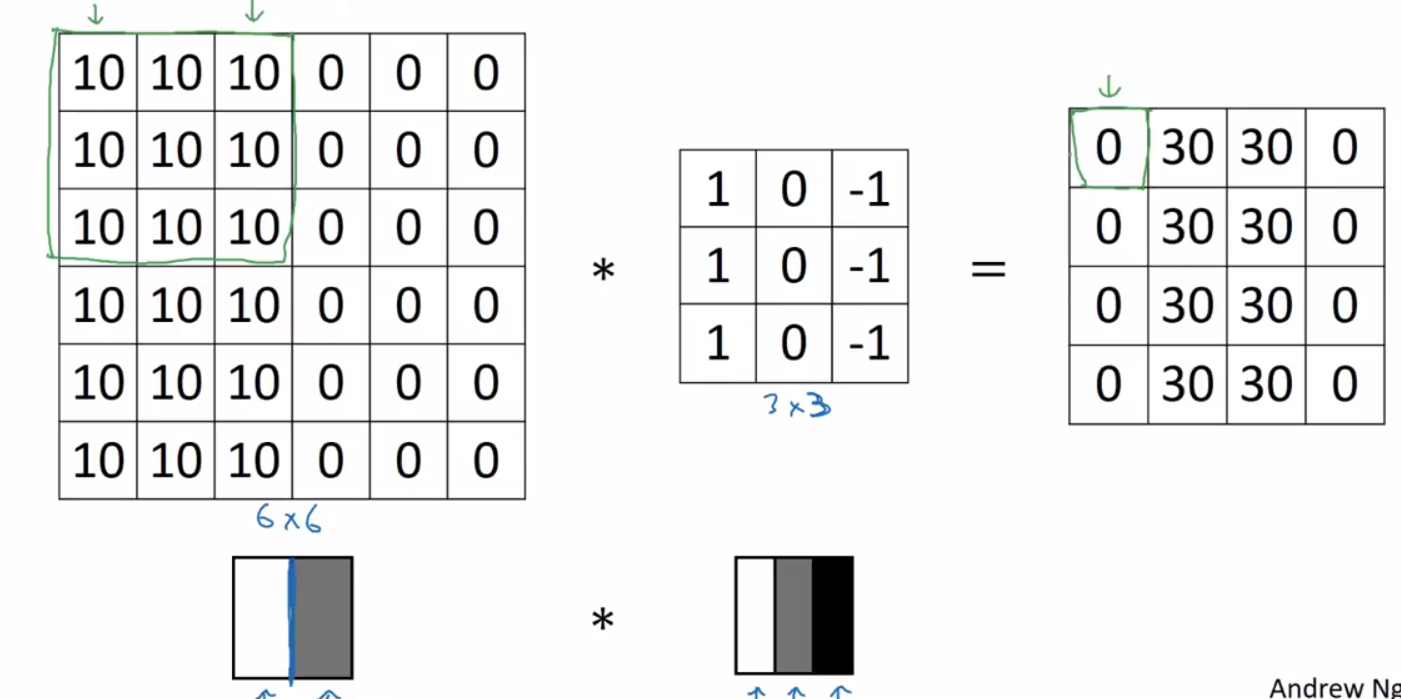
\includegraphics[width=0.6\textwidth]{esempio_convoluzione}
%     \caption{TODO Immagine da rifare}
%     \label{fig:conv_example}
%   \end{center}
% \end{figure}
%
% % TODO parentesi su il caso a colori?
% %%%%%%%%%%%%%%%%%%%%%%%%%%%%%%%%%%%%%%%%%%%%%%%%%%%%%%%%%%%%%%%%%%%%%%%%%%%%%%%%


\section{La Struttura di un Autoencoder}
\todo{Bisogna sistemare tutto da qua in poi}
% https://en.wikipedia.org/wiki/Autoencoder
% Struttura di un AE e differenze principali con CONV NN
Un Autoencoder (AE) è un particolare tipo di rete neurale il cui scopo è codificare efficacemente l'informazione fornita in input con modalità unsupervised.
Gli Autoencoder sono stati largamente utilizzati come tecniche per la dimensionality reduction, dimostrando capacità paragonabili a quelle di algoritmi come PCA o t-sne.
Un Autoencoder è formato da due componenti principali:
\begin{itemize}
    \item l'encoder, ottimizzato per generare una version compressa del dato;
    \item il decoder, ottimizzato per ricostruire l'informazione originale a partire dalla versione compressa.
\end{itemize}
Durante l'allenamento (training) la rete cerca di fornire un output il più simile possibile all'input ricevuto.
Potrebbe sembrare che l'obiettivo % TODO
dell'Autoencoder sia simulare la funzione identità, cioè quella funzione che fornisce in output esattamente l'input ricevuto.
In realtà all'interno della rete accade molto di più.
Prendiamo in esempio il più semplice degli AE: due layer fully-connected messi in sequenza.
Sappiamo che il numero di feature \footnote{TODO spiegare cosa si intende per feature} in ingresso nel primo layer deve combaciare con il numero di feature in uscita, altrimenti non potremmo confrontare l'input con la ricostruzione generata dalla rete.
Se si immaginano le feature in ingresso come dei punti, vettori, in un spazio n-dimensionale, con n pari al numero delle feature fornite, il compito dell'Autoencoder è generare dei punti che siano molto vicini ai punti osservati.
In altre parole si vuole che l'Autoencoder catturi la distribuzione probabilistica dei vettori forniti.
Stabilito, quindi, che la rete riceve e restituisce vettori di dimensionalità n si può definire la dimensionalità dello spazio latente, cioè di quello spazio di dimensione m, con $m < n$, in cui tutti i  vettori in input vengono mappati durante l'encoding.
Viene chiamato spazio latente perché non è conosciuto a priori.
Infatti sarà proprio la rete stessa, durante il training, a trovarlo, selezionandolo tra gli infiniti spazi m-dimensionali.
La dimensione dello spazio latente deve essere sufficientemente grande da permettere di mantenere le informazioni che caratterizzano l'input, ed allo stesso tempo sufficientemente piccolo così da rimuovere eventuale rumore o dati superflui.
Poco fa abbiamo definito due layer fully-connected, specificando soltanto le dimensioni in input del primo e le dimensioni in output del secondo.
Ora sappiamo che le feature in uscita dal primo layer dovranno essere accettate, in entrata, dal secondo.
Sappiamo anche che la dimensione della feature, in quanto vettore dello spazio latente, dovrà essere pari ad $m$.
La rete appena definita e raffigurata in %TODO figura
con la tipica forma a clessidra.
La parte più stretta di un Autoencoder è detta bottleneck (in italiano: collo di bottiglia) e corrisponde con la compressione massima del dato.

%TODO aggiungere formulazione matematica

\subsection{Variazioni dell'architettura}
Breve descrizione diconvAE stacked SAE DAE VAE


\subsection{Applicazioni principali}

La capacità degli Autoencoder di ricostruire l'input, quindi di mantenerne la struttura, privandolo di eventuale rumore o addirittura rimpiazzando il rumore con valori verosimili, si è rilevata utile in molti campi.

% TODO link ad anomaly detection
Quando il rumore incide notevolmente

% TODO link a paper image restoration
In questo paper si usano gli AE per colorare immagini un bg

Anche in questo documento la rimozione del rumore sarà un tema centrale, l'applicazione nel nostro caso verrà analizzato nel dettaglio nei prossimi capitoli.









\section {Convoluzioni e Convoluzioni Trasposte}
% Spiegazione dettagliata dei Conv Layers e dei Conv Transpose Layers
\section {Spazi Latenti}
% Sfruttabilità degli spazi latenti ed esempi di applicazioni

